\section{Traffic flow modelling}

\subsection{The LWR Model}

Lighthill and Whitham in 1955 \cite{Lighthill1955} introduce a macroscopic dynamic model of traffic based on conservation of cars (\ref{eq:LWRmodel1}), using Greenshields' hypothesis \cite{Greenshields1934} of a static flow/density relationship (\ref{eq:LWRmodel2}), known as the \textit{fundamental diagram}. The model consists of the following two equations:

\begin{equation} \label{eq:LWRmodel1}
\frac{\partial \rho(x,t)}{\partial t} + \frac{\partial q(x,t)}{\partial x} = 0
\end{equation}

\begin{equation} \label{eq:LWRmodel2}
q(x,t) = Q(\rho(x,t))
\end{equation}

\noindent where $\rho(x,t)$ and $q(x,t)$ denote the density and the flow of vehicles at location x and time t respectively, and $Q$ is the flux function which is assumed to be a function of the density only. 

Equation (\ref{eq:LWRmodel1}) is the principle of conservation of mass, or in this case conservation of vehicles, from fluid dynamics. These equations can be written more compactly as:

\begin{equation} \label{eq:LWRmodel3}
\frac{\partial \rho(x,t)}{\partial t} + Q'(\rho(x,t))\frac{\partial \rho(x,t)}{\partial x} = 0
\end{equation}

This equation is commonly known as the \textit{Lighthill-Whitham-Richards}, or LWR, model. Different fundamental diagrams have been suggested. Greenshields \cite{Greenshields1934} found that freeway speed and density could be reasonably well approximated by a straight line. The expression of the velocity and the flux are then:

\begin{equation} \label{eq:greenshieldsVelocity}
v = V_{G}(\rho) = v_{f}(1-\frac{\rho}{\rho_{\text{jam}}})
\end{equation}

\begin{equation} \label{eq:greenshieldsFlux}
Q_{G}(\rho) = \rho V_{G}(\rho) = v_{f}(\rho-\frac{\rho^{2}}{\rho_{\text{jam}}})
\end{equation}

where $v_{f}$ is the free flow (or maximum) velocity, and $\rho_{\text{jam}}$ is the jam (or maximum) density. In this case, the flow is a quadratic function of the density. 

Many researchers have later suggested alternative shapes that provide a better fit to the measured data. They all share the same characteristics \textbf{LWR1-6}:

LWR1. Greenshields' hypothesis of a static flow/density relationship: $q = Q(\rho(x,t))$

LWR2. $Q(0)=Q(\rho_{\text{jam}})$=0

LWR3. The continuous portions of $Q(\rho)$ are concave.

LWR4. $V(0) = v_{f}$, and $V(\rho_{\text{jam}}) = 0$.

LWR5. A critical density $\rho_{c}$ can be defined where the maximum flow $q_{c}$ is attained. Then, $Q(\rho)$ is increasing for $\rho \leq \rho_{c}$ and decrasing for $\rho > \rho_{c}$.

LWR6. The critical density $\rho_{c}$ separates the fundamental diagram into two regimes: \textit{free flow} when $\rho \leq \rho_{c}$ and \textit{congestion} when $\rho > \rho_{c}$

\begin{figure}[ht]
  \centering
    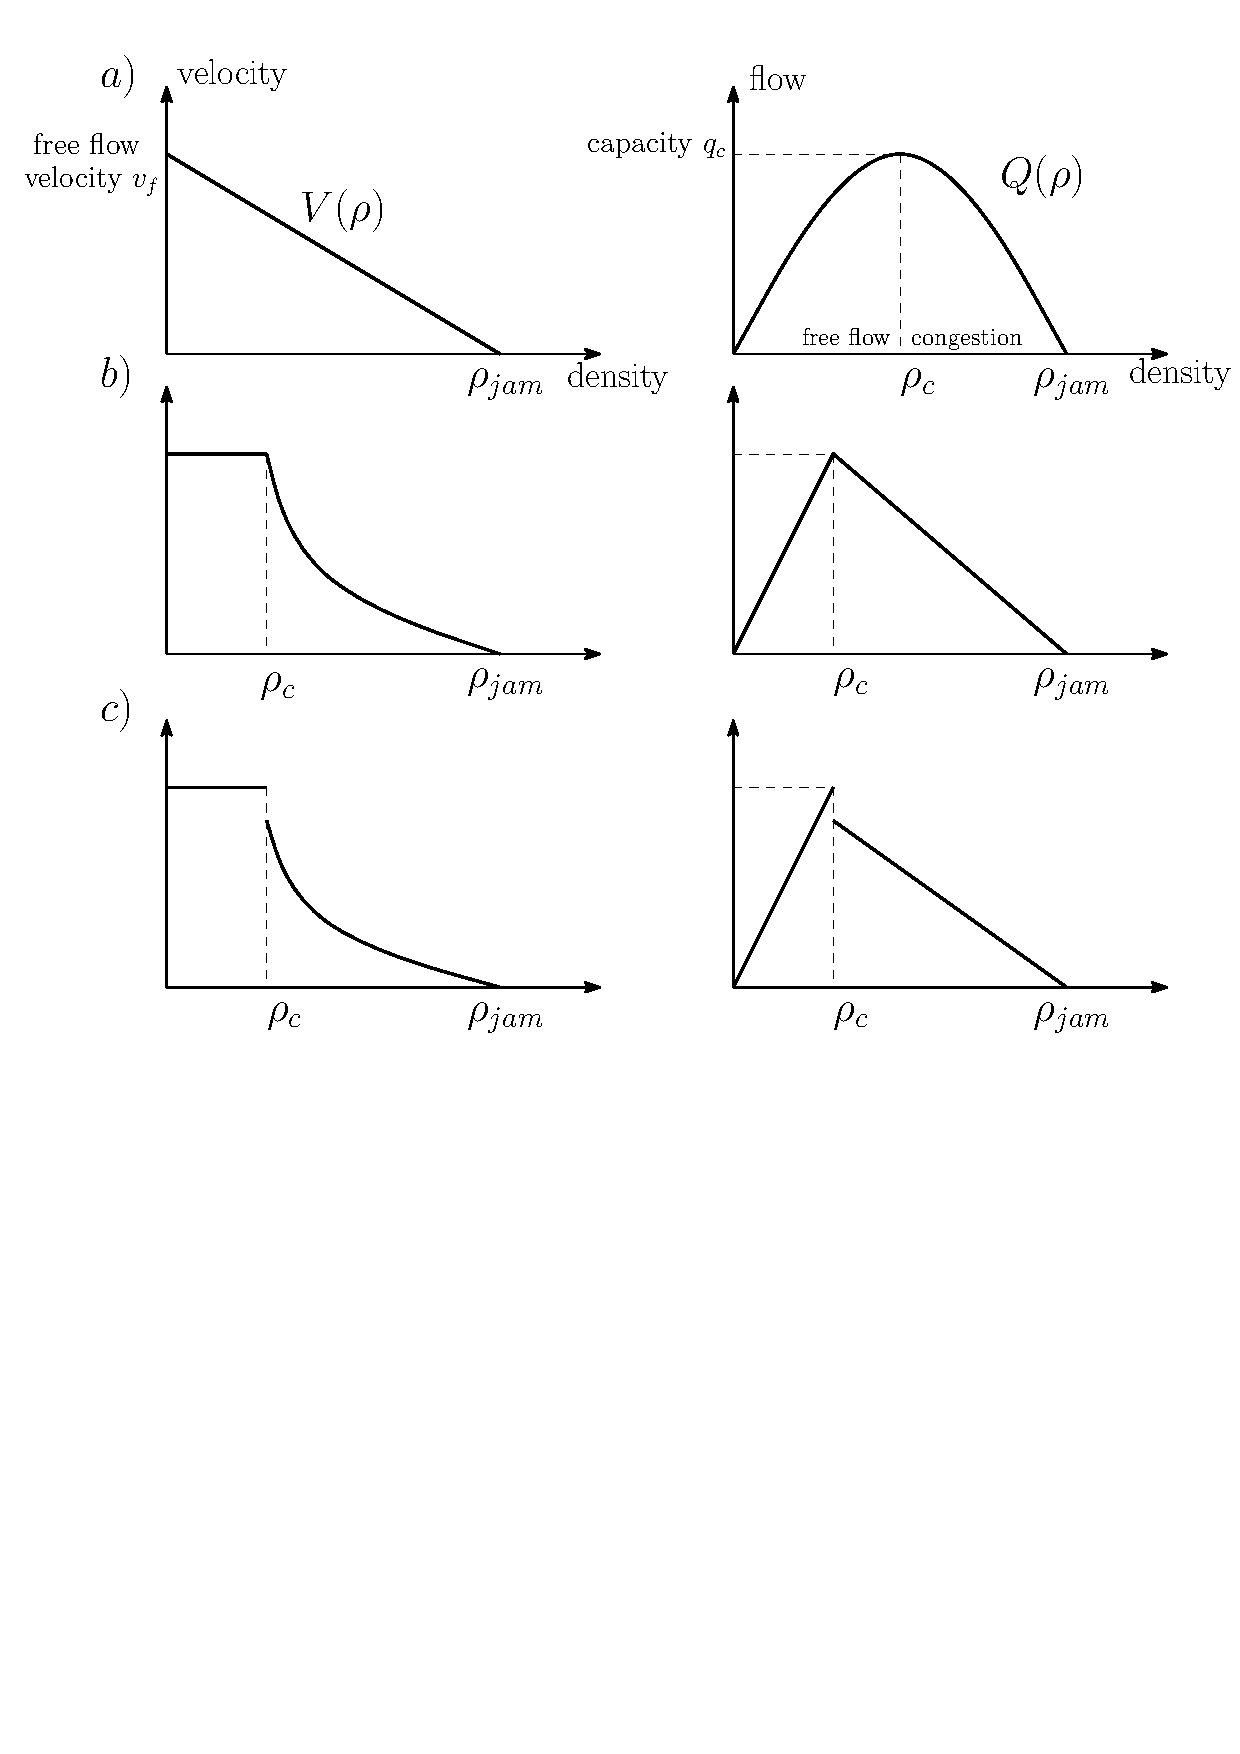
\includegraphics[width=8cm]{figures/fundamentalDiagram2.pdf}
    \caption{Speed and flow relationships (fundamental diagrams) for Greenshields (a), Daganzo-Newell (b), and discontinuous (c).}
    \label{fig:fundamentalDiagram}
\end{figure}

Many researchers have later suggested alternative shapes that provide a better fit to the measured data. For instance, the widely used Daganzo-Newell velocity function assumes a constant velocity in free-flow and a hyperbolic velocity in congestion as shown in Figure \ref{fig:fundamentalDiagram}:
\noindent 
\begin{equation}\label{eq:dnVelocity}
v = V_{DN}(\rho) = \begin{cases}
v_{f} & \text{if } \rho \leq \rho_{c} \\
-\omega_{f} \left( 1 - \frac{\rho_{\text{jam}}}{\rho} \right) & \text{if } \rho > \rho_{c}
\end{cases}
\end{equation}

\noindent and the corresponding flux function is:

\begin{equation}\label{eq:dnFlux}
\begin{array}{ll}
Q_{DN}(\rho) & = \rho V_{DN}(\rho)\\
 & = \begin{cases}
v_{f} \rho & \text{if } \rho \leq \rho_{c} \\
-\omega_{f} \left( \rho - \rho_{\text{jam}} \right) & \text{if } \rho > \rho_{c}
\end{cases}
\end{array}
\end{equation}

\noindent where $\omega_{f}=v_{f}\rho_{c}/(\rho_{\text{jam}}-\rho_{c})$ is the backwards propagation wave speed.

Measurements on the free-flow side are usually well represented by a straight line, whereas measurements in congestion tend to be more scattered. Some authors claim that there is a difference in the maximum measured flow $Q(\rho_{c})$, depending on whether the freeway is in free-flow or congestion, and contend that a \textit{discontinuity} exists at $\rho=\rho_{c}$ as in Figure \ref{fig:fundamentalDiagram}. This is described in \cite{Agyemang-Duah1991,Cassidy1999,Hall1991} as a \textit{capacity drop}, on the order of 4-10\% in peak flow, as the freeway transitions into congestion.

\subsection{Numerical Discretization}

A good numerical method to solve the equations along roads is represented by the Godunov scheme, which is based on exact solutions to Riemann problems \cite{Godlewski1996,Godunov1959}. This leads to the construction of a nonlinear discrete time dynamical system.

The Godunov discretization scheme is applied on the LWR PDE, where the discrete time step $\Delta t$ is indexed by $t$, and the discrete space step $\Delta x$ is indexed by $i$:

\begin{equation} \label{eq:rhoGodunov}
\rho^{t+1}_{i} = \rho^{t}_{i} - \frac{\Delta t}{\Delta x}\left(G(\rho^{t}_{i},\rho^{t}_{i+1})-G(\rho^{t}_{i-1},\rho^{t}_{i})\right)
\end{equation}

\noindent In order to ensure numerical stability, the time and space steps are coupled by the CFL condition \cite{LeVeque1992}: $c_{max}\frac{\Delta t}{\Delta x} \leq 1$ where $c_{max}$ denotes the maximal characteristic speed.

For a family of flux functions $Q(\rho)$ that share the same characteristics \textbf{LWR1-6} listed above, the Godunov flux can be expressed as the minimum of the \textit{sending flow} from the upstream cell and the \textit{receiving flow} from the downstream cell through a boundary connecting two cells of a homogeneous road (i.e. the upstream and downstream cells have the same characteristics) \footnotemark. The \textit{sending flow} $S(\rho)$ is equal to the upstream flow if the upstream traffic is in free flow ($\rho \leq \rho_{c}$) or the capacity of the upstream section $q_{c}$ if the upstream traffic is in congestion ($\rho > \rho_{c}$); on the other hand, the \textit{receiving flow} $R(\rho)$ is equal to the capacity of the downstream section if the downstream traffic is in free flow or the downstream flow if the downstream traffic is in congestion. For this model, we note that for an heterogeneous segment (for instance due to a change in the number of lanes) a fundamental diagram with different parameters is defined at each cell $i$, consequently we add a subscript: $Q_{i}(\rho)$, $S_{i}(\rho)$, $R_{i}(\rho)$ and there is an implicit subscript for $G(\rho_{i},\rho_{i+1})$.

\footnotetext{
There are various definitions of the Godunov flux $G(\rho_{1},\rho_{2})$ in the literature, notably in \cite{Garavello2006}:

\begin{equation} \label{eq:rhoGodunovFluxGeneral}
G(\rho_{1},\rho_{2}) = \begin{cases}
\text{min}_{\rho \in [\rho_{1},\rho_{2}]} Q(\rho) & \text{if } \rho_{1} \leq \rho_{2}\\
\text{max}_{\rho \in [\rho_{2},\rho_{1}]} Q(\rho) & \text{if } \rho_{2} \leq \rho_{1}
\end{cases}
\end{equation}
\noindent This assumes that a fundamental diagram is defined at each boundary between two cells, which differs from the CTM.
}

\begin{equation} \label{eq:rhoGodunovFlux1}
G(\rho_{1},\rho_{2}) = \text{min}(S_{1}(\rho_{1}),R_{2}(\rho_{2}))
\end{equation}

\begin{equation} \label{eq:sendingFlow1}
S_{1}(\rho) = \begin{cases}
Q_{1}(\rho) & \text{if } \rho \leq \rho_{c1} \\
q_{c1} &  \text{if } \rho > \rho_{c1}
\end{cases}
\end{equation}

\begin{equation} \label{eq:receivingFlow1}
R_{2}(\rho) = \begin{cases}
q_{c2} & \text{if } \rho \leq \rho_{c2} \\
Q_{2}(\rho) &  \text{if } \rho > \rho_{c2}
\end{cases}
\end{equation}

\noindent where $\rho_{1}$ is the density of the cell upstream and $\rho_{2}$ is the density of the cell downstream. Then sending and receiving flows for the Daganzo-Newell fundamental diagram is:

\begin{equation} \label{eq:sendingFlow2}
S_{1}(\rho) = \begin{cases}
v_{f1}\rho & \text{if } \rho \leq \rho_{c1} \\
q_{c1} &  \text{if } \rho > \rho_{c1}
\end{cases}
\end{equation}

\begin{equation} \label{eq:receivingFlow2}
R_{2}(\rho) = \begin{cases}
q_{c2} & \text{if } \rho \leq \rho_{c2} \\
-\omega_{f2} \left( \rho - \rho_{\text{jam}2} \right) & \text{if } \rho > \rho_{c2}
\end{cases}
\end{equation}

\begin{figure}[ht]
  \centering
    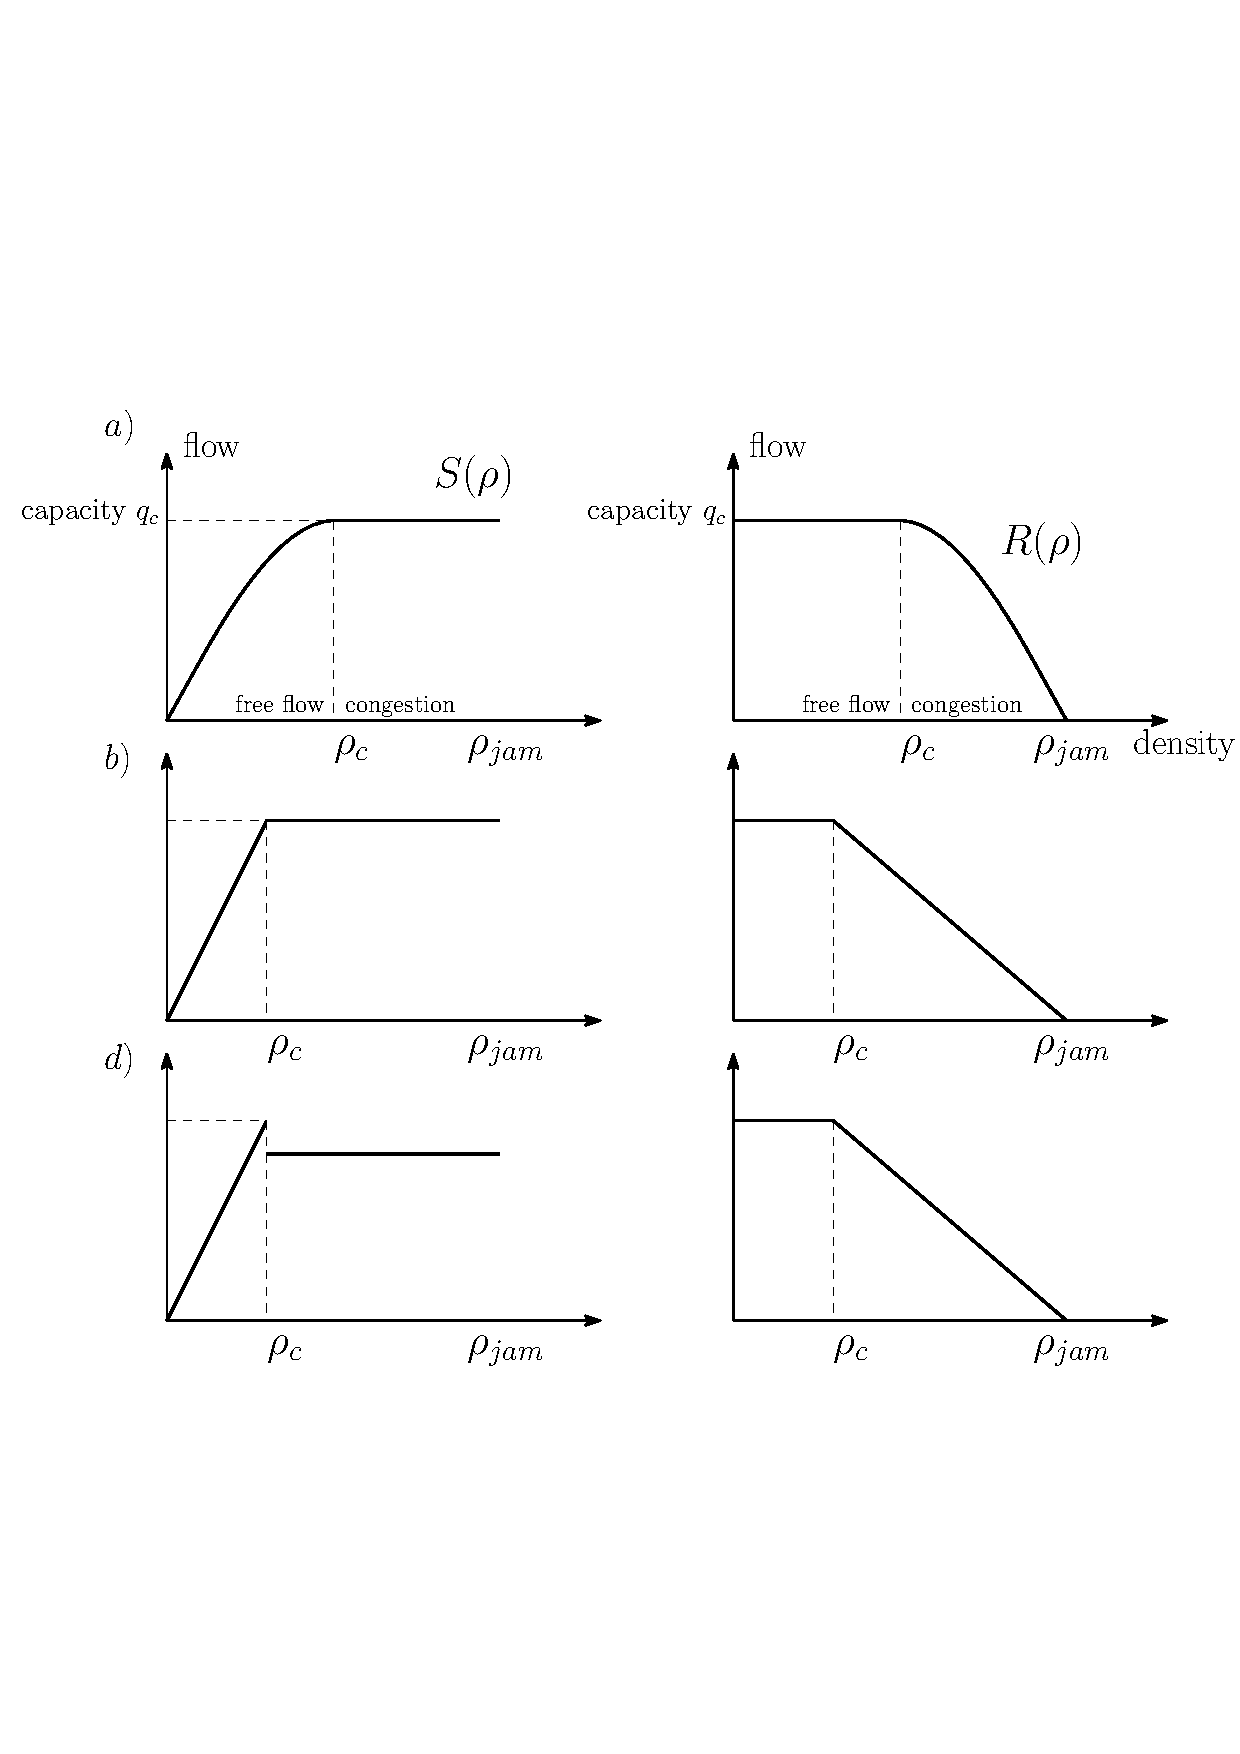
\includegraphics[width=8cm]{figures/fundamentalDiagramSR.pdf}
    \caption{Sending and receiving flows for Greenshields (a), Daganzo-Newell (b), and discontinous (c) velocity functions.}
    \label{fig:fundamentalDiagramSR}
\end{figure}

\noindent As shown in Figure \ref{fig:fundamentalDiagramSR}, the application of the Godunov scheme to the fundamental diagrams introduces intuitive concepts of \textit{supply} and \textit{demand} at the boundary connecting two cells. The upstream cell supplies the flow at the boundary up to capicity. We can note that in the discontinuous case, there is a drop in supply capacity when the upstream traffic is in congestion, as described in \cite{Agyemang-Duah1991,Cassidy1999,Hall1991}. As a result, the flow through the boundary is smaller, even if the downstream cell can receive more flow. On the other hand, when the downstream traffic is congested, there is a decrease in demand from the downstream cell, limiting the flow through the boundary.

\hspace{10mm}

\noindent\textbf{Important remark:} For the rest of the paper, the widely-used \textit{Cell Transmission Model} (CTM) described in \cite{Daganzo1994} is chosen for our dynamic model and results are derived from it. We also suppose for simplicity and clarity that the segment of road we are modelling is homogeneous, i.e. the parameters of the fundamental diagram $\omega_{f}$, $v_{f}$, $\rho_{\text{jam}}$, $\rho_{c}$, $q_{c}$ are constant along the cells of the discretized road. And they are also time invariant because they are only related to the geometry of the highway, independently of the current traffic on it. All the results derived in the rest of the paper still remain for an heterogeneous road, in particular the piecewise affine character of the model and the tractibility of the Kalman filter algorithm, but the number of modes and the complexity increase. For more details on the heterogeneous case, see Appendix \ref{sec:CDFD}.

\hspace{10mm}

\noindent Figure \ref{fig:godunovDiagram} shows the explicit values taken by $G(\rho_{1},\rho_{2})$ for a partition of the space in different regions of the space $(\rho_{1},\rho_{2})$. We will denote by \textbf{W}, \textbf{L}, and \textbf{D} the \textit{white region}, \textit{light region}, and \textit{dark region} of the space $(\rho_{1},\rho_{2})$ respectively. 

\begin{equation}
G(\rho_{1},\rho_{2}) = \begin{cases}
R(\rho_{2}) & \text{if } (\rho_{1},\rho_{2}) \in \textbf{W}\\
q_{c} & \text{if } (\rho_{1},\rho_{2}) \in \textbf{L}\\
S(\rho_{1}) & \text{if } (\rho_{1},\rho_{2}) \in \textbf{D}
\end{cases}
\label{eq:rhoGodunovFlux}
\end{equation}

\begin{equation}
\begin{array}{ll}
\textbf{W} & = \{(\rho_{1},\rho_{2}) \mid \rho_{2} > F(\rho_{1}) \text{ ,   } \rho_{2} > \rho_{c}\}\\
\textbf{L} & = \{(\rho_{1},\rho_{2}) \mid \rho_{1} > \rho_{c} \text{ ,   } \rho_{2} \leq \rho_{c}\}\\
\textbf{D} & = \{(\rho_{1},\rho_{2}) \mid \rho_{2} \leq F(\rho_{1}) \text{ ,   } \rho_{1} \leq \rho_{c}\}
\end{array}
\label{eq:regions}
\end{equation}

\noindent where the boundary between the white and grey regions follows the $(\rho_{1},\rho_{2})=(\rho_{1},F(\rho_{1}))$ trajectory with $F(\rho_{1})= \bar{R}^{-1}(\bar{S}(\rho_{1}))$\footnotemark for $\rho_{1} \leq \rho_{c}$. $\bar{S}$ and $\bar{R}$ denote the restrictions of the sending and receiving flows to the sub-regions $[0,\rho_{c})$ and $(\rho_{c},\rho_{\text{jam}}]$ respectively, which also correspond to the left and right parts (w.r.t. $\rho_{c}$) of the fundamental diagram, as shown in the Figure \ref{fig:godunovDiagram}.

\footnotetext{Here, we formulate the more general case for equations (\ref{eq:rhoGodunovFlux}, \ref{eq:regions}) and we suppose that $\bar{R}$ is a strictly monotonic function on $(\rho_{c},\rho_{j}]$, hence invertible, and $\bar{R}^{-1}$ denotes its inverse, which is the case for the Daganzo-Newell fundamental diagram.}

\begin{figure}[ht]
  \centering
    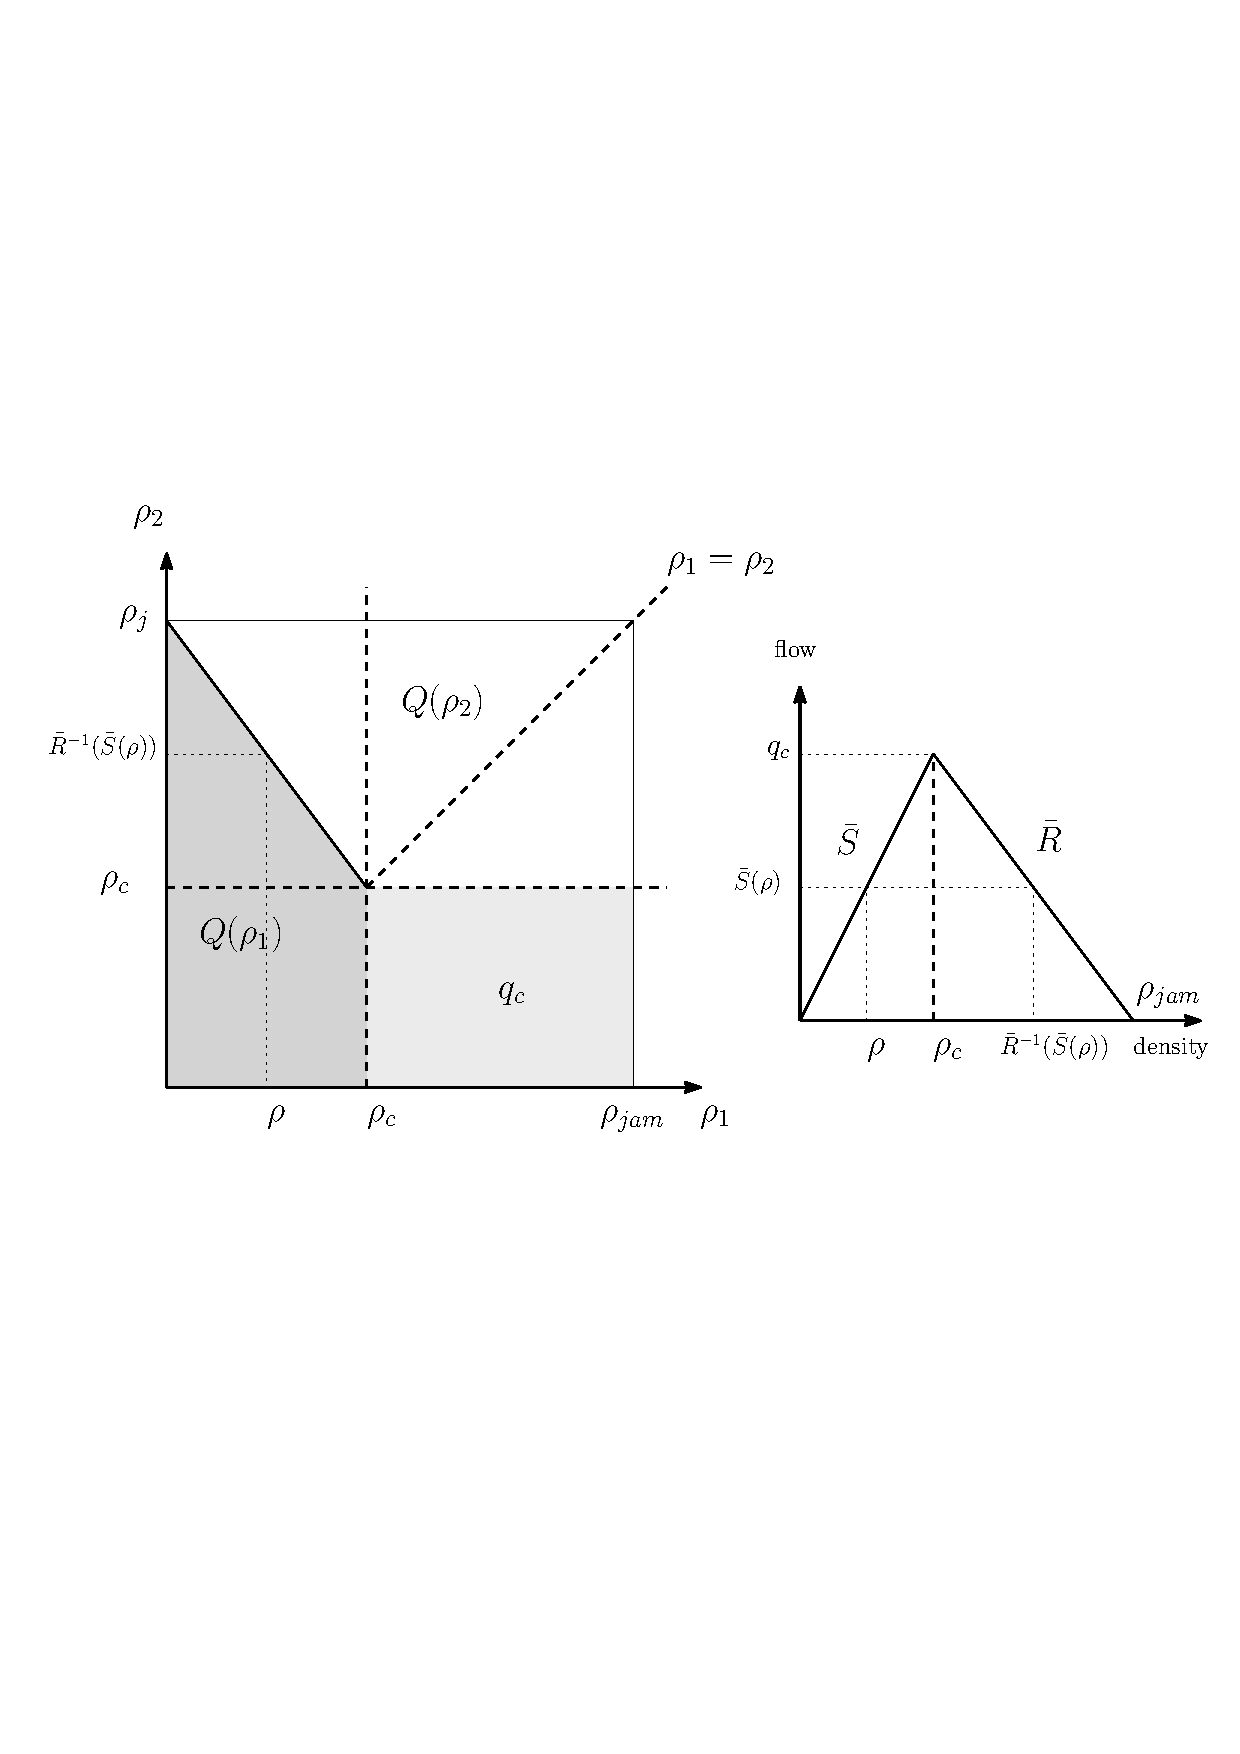
\includegraphics[width=8cm]{figures/godunovDiagram.pdf}
    \caption{Values of $G(\rho_{1},\rho_{2})$ in the space $(\rho_{1},\rho_{2})$.}
    \label{fig:godunovDiagram}
\end{figure}

\noindent When the velocity is the Daganzo-Newell function (\ref{eq:dnVelocity}), the Godunov Flux becomes:
\begin{equation} \label{eq:rhoGodunovFlux3}
\begin{array}{l}
G_{DN}(\rho_{1},\rho_{2})\\
= \begin{cases}
-\omega_{f} \left( \rho_{2} - \rho_{\text{jam}} \right) & \text{if } (\rho_{1},\rho_{2}) \in \textbf{W}\\
q_{c} & \text{if } (\rho_{1},\rho_{2}) \in \textbf{L}\\
v_{f} \rho_{1} & \text{if } (\rho_{1},\rho_{2}) \in \textbf{D}
\end{cases}
\end{array}
\end{equation}

\noindent and the boundary between \textbf{W} and \textbf{D} regions is:

\begin{equation} \label{eq:boundary}
(\rho_{1},\rho_{2})=(\rho_{1},-\frac{v_{f}}{\omega_{f}}\rho_{1}+\rho_{\text{jam}})
\end{equation}

\noindent And \textbf{W}, \textbf{L}, \textbf{D} form a \textit{polyhedral partition} of the space $(\rho_{1},\rho_{2})$:

\begin{equation}
\begin{array}{ll}
\textbf{W} & = \{(\rho_{1},\rho_{2}) \mid \rho_{2} + \frac{v_{f}}{\omega_{f}}\rho_{1} > \rho_{\text{jam}} \text{ ,   } \rho_{2} > \rho_{c}\}\\
\textbf{L} & = \{(\rho_{1},\rho_{2}) \mid \rho_{1} > \rho_{c} \text{ ,   } \rho_{2} \leq \rho_{c}\}\\
\textbf{D} & = \{(\rho_{1},\rho_{2}) \mid \rho_{2} + \frac{v_{f}}{\omega_{f}}\rho_{1} \leq \rho_{\text{jam}} \text{ ,   } \rho_{1} \leq \rho_{c}\}\end{array}
\label{eq:regions2}
\end{equation}